\documentclass[tikz,border=8pt]{standalone}
% Shared look for every TikZ diagram. Load with \input{../../tools/tikz-style.tex}
\usepackage[sfdefault]{roboto}
\usetikzlibrary{arrows.meta, positioning, shapes.geometric, calc, fit, backgrounds}
\definecolor{cblue}{HTML}{4C78A8}
\definecolor{corange}{HTML}{F58518}
\definecolor{cgreen}{HTML}{54A24B}
\definecolor{cred}{HTML}{E45756}
\definecolor{cpurple}{HTML}{B279A2}
\definecolor{cgrey}{HTML}{6B6B6B}
\tikzset{
  every picture/.style={font=\sffamily, line width=1.2pt},
  box/.style={draw=#1, fill=#1!12, rounded corners=4pt, align=center, inner sep=7pt, minimum height=1.1cm},
  box/.default=cgrey,
  arrow/.style={-{Stealth[length=3mm]}, draw=cgrey, line width=1.4pt},
  title/.style={font=\sffamily\bfseries\Large},
  note/.style={font=\sffamily\small, text=cgrey, align=center},
}
\AtBeginDocument{\hyphenpenalty=10000 \exhyphenpenalty=10000}

% The plant split in two: the actuator (the drive, which can give at most 4 N) and the process (the robot's body).
% Numbers at the moment the held robot is let go (t = 5 s): the controller asks for c = 25.9 N, the drive gives u = 4 N.
\begin{document}
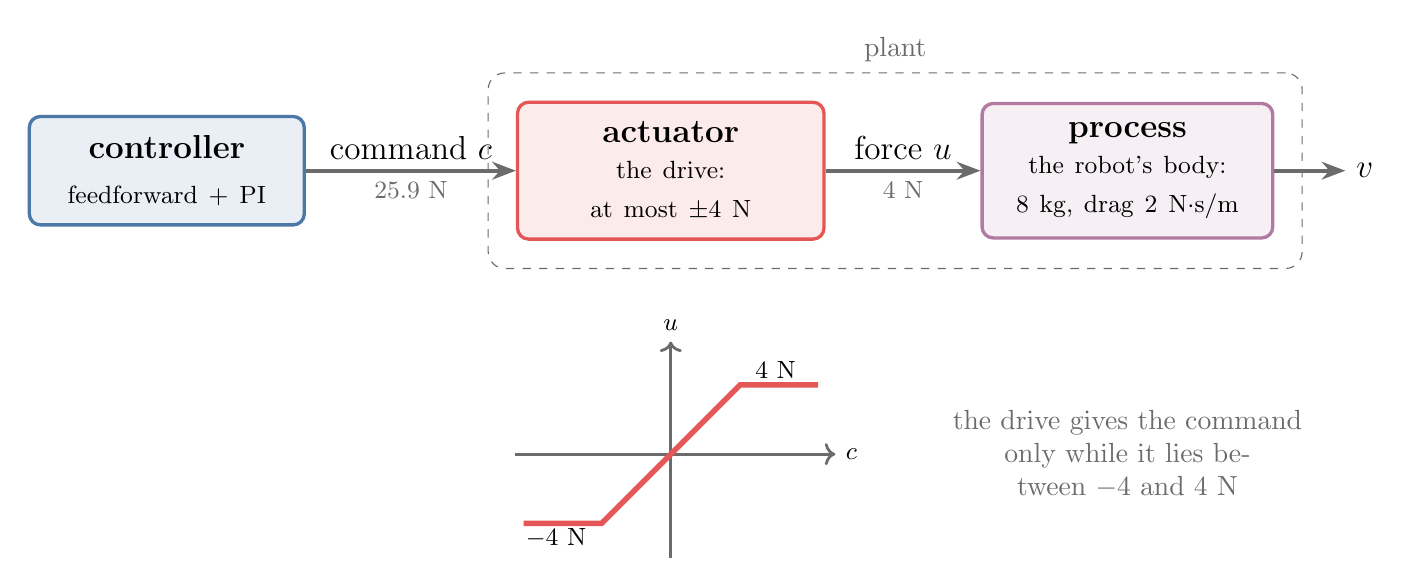
\begin{tikzpicture}[every node/.append style={font=\large}]
  \node[box=cblue, text width=3.0cm] (ctrl) at (0,0) {\textbf{controller}\\[2pt] \small feedforward + PI};
  \node[box=cred, text width=3.4cm] (act) at (6.4,0) {\textbf{actuator}\\[2pt] \small the drive:\\ at most $\pm$4 N};
  \node[box=cpurple, text width=3.2cm] (proc) at (12.2,0) {\textbf{process}\\[2pt] \small the robot's body:\\
     8 kg, drag 2 N$\cdot$s/m};
  \draw[arrow] (ctrl) -- node[above] {command $c$} node[below, font=\small, text=cgrey] {25.9 N} (act);
  \draw[arrow] (act) -- node[above] {force $u$} node[below, font=\small, text=cgrey] {4 N} (proc);
  \draw[arrow] (proc.east) -- ++(0.9,0) node[right] {$v$};
  \begin{scope}[on background layer]
    \node[draw=cgrey, dashed, rounded corners=6pt, inner sep=10pt, fit=(act) (proc)] (plant) {};
  \end{scope}
  \node[note, font=\normalsize, anchor=south] at (plant.north) {plant};
  % the drive's input-output curve: a line that flattens at +-4 N
  \begin{scope}[shift={(6.4,-3.6)}, scale=0.55]
    \draw[->, cgrey, line width=1pt] (-3.6,0) -- (3.8,0) node[right, font=\small, text=black] {$c$};
    \draw[->, cgrey, line width=1pt] (0,-2.4) -- (0,2.6) node[above, font=\small, text=black] {$u$};
    \draw[cred, line width=2pt] (-3.4,-1.6) -- (-1.6,-1.6) -- (1.6,1.6) -- (3.4,1.6);
    \node[font=\small, anchor=west] at (1.7,1.95) {4 N};
    \node[font=\small, anchor=east] at (-1.7,-1.95) {$-$4 N};
  \end{scope}
  \node[note, font=\normalsize, text width=4.6cm] at (12.2,-3.6) {the drive gives the command\\ only while it lies
     between $-$4 and 4 N};
\end{tikzpicture}
\end{document}
